%% Copernicus Publications Manuscript Preparation Template for LaTeX Submissions
%% ---------------------------------
%% This template should be used for copernicus.cls
%% The class file and some style files are bundled in the Copernicus Latex Package, which can be downloaded from the different journal webpages.
%% For further assistance please contact Copernicus Publications at: production@copernicus.org
%% https://publications.copernicus.org/for_authors/manuscript_preparation.html

%% copernicus_rticles_template (flag for rticles template detection - do not remove!)

%% Please use the following documentclass and journal abbreviations for discussion papers and final revised papers.

%% 2-column papers and discussion papers
\documentclass[gc, manuscript]{copernicus}



%% Journal abbreviations (please use the same for discussion papers and final revised papers)


% Advances in Geosciences (adgeo)
% Advances in Radio Science (ars)
% Advances in Science and Research (asr)
% Advances in Statistical Climatology, Meteorology and Oceanography (ascmo)
% Annales Geophysicae (angeo)
% Archives Animal Breeding (aab)
% ASTRA Proceedings (ap)
% Atmospheric Chemistry and Physics (acp)
% Atmospheric Measurement Techniques (amt)
% Biogeosciences (bg)
% Climate of the Past (cp)
% DEUQUA Special Publications (deuquasp)
% Drinking Water Engineering and Science (dwes)
% Earth Surface Dynamics (esurf)
% Earth System Dynamics (esd)
% Earth System Science Data (essd)
% E&G Quaternary Science Journal (egqsj)
% Fossil Record (fr)
% Geochronology (gchron)
% Geographica Helvetica (gh)
% Geoscience Communication (gc)
% Geoscientific Instrumentation, Methods and Data Systems (gi)
% Geoscientific Model Development (gmd)
% History of Geo- and Space Sciences (hgss)
% Hydrology and Earth System Sciences (hess)
% Journal of Micropalaeontology (jm)
% Journal of Sensors and Sensor Systems (jsss)
% Mechanical Sciences (ms)
% Natural Hazards and Earth System Sciences (nhess)
% Nonlinear Processes in Geophysics (npg)
% Ocean Science (os)
% Primate Biology (pb)
% Proceedings of the International Association of Hydrological Sciences (piahs)
% Scientific Drilling (sd)
% SOIL (soil)
% Solid Earth (se)
% The Cryosphere (tc)
% Web Ecology (we)
% Wind Energy Science (wes)


%% \usepackage commands included in the copernicus.cls:
%\usepackage[german, english]{babel}
%\usepackage{tabularx}
%\usepackage{cancel}
%\usepackage{multirow}
%\usepackage{supertabular}
%\usepackage{algorithmic}
%\usepackage{algorithm}
%\usepackage{amsthm}
%\usepackage{float}
%\usepackage{subfig}
%\usepackage{rotating}


% The "Technical instructions for LaTex" by Copernicus require _not_ to insert any additional packages.
%
\usepackage{algorithmic}
\usepackage{algorithm}

\usepackage{color}
\usepackage{fancyvrb}
\newcommand{\VerbBar}{|}
\newcommand{\VERB}{\Verb[commandchars=\\\{\}]}
\DefineVerbatimEnvironment{Highlighting}{Verbatim}{commandchars=\\\{\}}
% Add ',fontsize=\small' for more characters per line
\usepackage{framed}
\definecolor{shadecolor}{RGB}{248,248,248}
\newenvironment{Shaded}{\begin{snugshade}}{\end{snugshade}}
\newcommand{\AlertTok}[1]{\textcolor[rgb]{0.94,0.16,0.16}{#1}}
\newcommand{\AnnotationTok}[1]{\textcolor[rgb]{0.56,0.35,0.01}{\textbf{\textit{#1}}}}
\newcommand{\AttributeTok}[1]{\textcolor[rgb]{0.77,0.63,0.00}{#1}}
\newcommand{\BaseNTok}[1]{\textcolor[rgb]{0.00,0.00,0.81}{#1}}
\newcommand{\BuiltInTok}[1]{#1}
\newcommand{\CharTok}[1]{\textcolor[rgb]{0.31,0.60,0.02}{#1}}
\newcommand{\CommentTok}[1]{\textcolor[rgb]{0.56,0.35,0.01}{\textit{#1}}}
\newcommand{\CommentVarTok}[1]{\textcolor[rgb]{0.56,0.35,0.01}{\textbf{\textit{#1}}}}
\newcommand{\ConstantTok}[1]{\textcolor[rgb]{0.00,0.00,0.00}{#1}}
\newcommand{\ControlFlowTok}[1]{\textcolor[rgb]{0.13,0.29,0.53}{\textbf{#1}}}
\newcommand{\DataTypeTok}[1]{\textcolor[rgb]{0.13,0.29,0.53}{#1}}
\newcommand{\DecValTok}[1]{\textcolor[rgb]{0.00,0.00,0.81}{#1}}
\newcommand{\DocumentationTok}[1]{\textcolor[rgb]{0.56,0.35,0.01}{\textbf{\textit{#1}}}}
\newcommand{\ErrorTok}[1]{\textcolor[rgb]{0.64,0.00,0.00}{\textbf{#1}}}
\newcommand{\ExtensionTok}[1]{#1}
\newcommand{\FloatTok}[1]{\textcolor[rgb]{0.00,0.00,0.81}{#1}}
\newcommand{\FunctionTok}[1]{\textcolor[rgb]{0.00,0.00,0.00}{#1}}
\newcommand{\ImportTok}[1]{#1}
\newcommand{\InformationTok}[1]{\textcolor[rgb]{0.56,0.35,0.01}{\textbf{\textit{#1}}}}
\newcommand{\KeywordTok}[1]{\textcolor[rgb]{0.13,0.29,0.53}{\textbf{#1}}}
\newcommand{\NormalTok}[1]{#1}
\newcommand{\OperatorTok}[1]{\textcolor[rgb]{0.81,0.36,0.00}{\textbf{#1}}}
\newcommand{\OtherTok}[1]{\textcolor[rgb]{0.56,0.35,0.01}{#1}}
\newcommand{\PreprocessorTok}[1]{\textcolor[rgb]{0.56,0.35,0.01}{\textit{#1}}}
\newcommand{\RegionMarkerTok}[1]{#1}
\newcommand{\SpecialCharTok}[1]{\textcolor[rgb]{0.00,0.00,0.00}{#1}}
\newcommand{\SpecialStringTok}[1]{\textcolor[rgb]{0.31,0.60,0.02}{#1}}
\newcommand{\StringTok}[1]{\textcolor[rgb]{0.31,0.60,0.02}{#1}}
\newcommand{\VariableTok}[1]{\textcolor[rgb]{0.00,0.00,0.00}{#1}}
\newcommand{\VerbatimStringTok}[1]{\textcolor[rgb]{0.31,0.60,0.02}{#1}}
\newcommand{\WarningTok}[1]{\textcolor[rgb]{0.56,0.35,0.01}{\textbf{\textit{#1}}}}

\begin{document}

\title{Management induced changes of soil organic carbon on global croplands \newline or \newline How management changed soil organic carbon on global croplands \newline or \newline Agricultural soil have lost 13 GtC topsoil carbon \newline or \newline Linking agricultural management data to soil modeleling -- a global approach}


\Author[1]{Kristine}{Karstens}
\Author[1]{Benjamin Leon}{Bodirsky}
\Author[2]{Your}{Name}
\Author[1]{Alexander}{Popp}


\affil[1]{Potsdam-Institut of Climate Impacts Research, Potsdam, Germany}
\affil[2]{Your affiliation}

%% The [] brackets identify the author with the corresponding affiliation. 1, 2, 3, etc. should be inserted.



\runningtitle{R Markdown Template for Copernicus}

\runningauthor{Nüst et al.}


\correspondence{Kristine\ Karstens\ (\href{mailto:kristine.karstens@pik-potsdam.de}{\nolinkurl{kristine.karstens@pik-potsdam.de}})}



\received{}
\pubdiscuss{} %% only important for two-stage journals
\revised{}
\accepted{}
\published{}

%% These dates will be inserted by Copernicus Publications during the typesetting process.


\firstpage{1}

\maketitle


\begin{abstract}
Soil organic carbon (SOC) is one of larges c stocks on earth (3 times larger biosphere pool).
\end{abstract}


\copyrightstatement{The author's copyright for this publication is transferred to institution/company.}


\newpage

\introduction

The depletion of soil organic carbon (SOC) due agricultural management has been a major source of carbon emissions, but also offers the potential to turn into a large additional carbon sink and thus mitigate climate change. Whereas the extent of the sink potential by SOC enhancement is highly debated (add refs), it is largely agreed upon that the SOC pool itself is the biggest terrestrial carbon pool, exceeding the atmospheric and even more the biospheric carbon pool multiple times. Even small changes in SOC drivers might lead to substantial shifts in earth carbon cycled and influence the atmospheric CO2 concentration (ref. permafrost melting). The specific amount of carbon stored in the soil is uncertain though and estimates ranging from 1500 to 2400 GtC for the first meter of the soil profile (Bathjes, 1996).

Mapping the worlds SOC has been investigated intensivly over the last decades and led to an increased quality of SOC maps as well as a even better understanding of factors driving magnitude, distribution and dynamics of SOC pools. Natural properties like climatic, biophysical and landscape characteristics clearly play the most important role in this regard.

Human intervention, including land cover change and land management, has however added a further driver to SOC change, which alters terrestrial carbon pools in much shorter time scales and is likely the dominant driver of SOC change on managed land today. Recent studies identified the anthropogenic SOC debt at around 116 GtC (Sanderman et al.), which compares to older estimates of around 60-130 GtC (Lal, 2006). Other studies have focused more closely on spatial disaggregated SOC changes via advanced digital soil mapping techniques (S-World; Stoorvogel 2, 2017) or better representation of biogeochemcial processes within SOC dynamics (). Despite providing a rough estimate of the order of magnitude of change, these studies lack a detailed consideration of land management.

Field-scale models (ref. Daycent, RothC, Ecosse, C-Tool) are able to capture these land mangement impacts by using detailed information on yield levels, fertilizer inputs and various other on farming activities. Yet, due to the lack of comprehensive global management data to feed these input demanding models, it seems still very complex to scale them up to a global extent.

Our study combines an spatial-explicit estimate of agricultural management data on global level with a robust but light weighted SOC model to estimate SOC stocks and stock change factors as well as organic carbon flow dynamics within the agricultural system. We thereby consider change in SOC caused by historical land cover change as well as of different agricultural mangement practices, including residue recycling, manure amendments, irrigation and tillage. We thereby provide the first global, spatial explicit SOC maps that consider agricultural management.

This paper will introduce in the the first part of the method section the basic concept of SOC dynamics. We continue in the second part with a detailed description of the used global gridded management data on production levels, residue recycling rates, manure amendments, irrigation and tillage adoption. In a third, small part, we shortly refer to the concept of stock change factors as outlined in the Tier 1 approach of the IPCC guidelines.
In our result section we will focus on the SOC dynamics on global croplands by analysing (1) the spatial explicit SOC distribution and depletion over the last decades, (2) compare the climate zone specfic stock changes with default stock changes factors from the IPCC Tier 1 approach and (3) compare global agricultrual carbon flows and stocks to contextualize the importants of the different management aspects.
Finally, we will discuss our findings and their implications on SOC model development and conlude with an analysis and outlook on the the opportunities for SOC management for climate change mitigation and negative emissions.

\newpage

\hypertarget{method-50}{%
\section{Method (50)}\label{method-50}}

We compiled calculations as open-source R packages available under github.com/pik-piam/mrcommons (management related functions) and github.com/pik-piam/mrSOCbudget (soil dynamic related functions), which are both based on github.com/pik-piam/madrat, a framework improving reproducibility and transparency in data processing.
In the following chapter we outine the most important relationships and assumptions. See table \ref{append:subsection2mrfunctions} for further information on corresponding code within the R packages.

\hypertarget{sec:carbonbudget}{%
\subsection{Carbon Stocks following (new) Tier 2 method (50)}\label{sec:carbonbudget}}

Following the tier 2 approach of the refinement of IPCC guidelines vol.~4 (\citet{ipcc_2019_2019}), we estimate soil organic carbon (SOC) stocks for cropland and all other land represented by natural vegetation on half-degree resolution from 1975 to 2010. We assume the actual SOC state converges towards a stable steady state, that itself is changing over time and space depending on biophysical, climatic and agronomic conditions. Therefore we conduct the following three steps within each yearly timestep:
(1) We calculate annual land-use (sub-)type specific steady states and decay rates for SOC stocks,
(2) We account for land conversion by transferring SOC between land-use types and
(3) We estimate SOC stocks based on the stocks of the previous time period, the steady state stocks and the decay rate.

\hypertarget{steady-state-soc-stocks-and-decay-rates}{%
\subsubsection{Steady-state SOC stocks and decay rates}\label{steady-state-soc-stocks-and-decay-rates}}

In a simple first order kinetic approach the steady-state soil organic carbon stocks \(SOC^{eq}\) are given by
\begin{equation}
SOC^{eq} =\frac{C^{\textrm{in}}}{k} \qquad\forall\quad i,t
\label{eq:inoutflow}
\end{equation}
with \(C^{\textrm{in}}\) being carbon inputs to the soil, \(k\) denoting the soil organic carbon decay rate; as well as \(i\) representing grid cells indecies and \(t\) years. We use for our calculations the steady-state method of the refinement of the IPCC guidelines vol.~4 (\citet{ipcc_2019_2019}) for mineral soils, which assume three soil carbon sub-pools (active, slow and passive) and entangled dynamics between them. Annual carbon inflow to each sub-pool (see \ref{sec:carboninputs}) and annual decay rates (see \ref{sec:tier2}) of each sub-pool are still the key components to determining steady-state SOC stocks.

\hypertarget{carbon-inputs-to-the-soil-seccarboninputs}{%
\paragraph*{Carbon Inputs to the Soil \{\#sec:carboninputs\}}\label{carbon-inputs-to-the-soil-seccarboninputs}}
\addcontentsline{toc}{paragraph}{Carbon Inputs to the Soil \{\#sec:carboninputs\}}

We account for different carbon input sources depending on our two distinguished land-use types (see table \ref{tab:datasourceinputs}); in particular for recycled crop residues, below ground biomass of crops (for both see \ref{sec:residues}) and recycled manure (see @ref(sec:livst\_manure)) on croplands; and litterfall (\citep{LPJmL4_1}) on natural vegetation.

Following the IPCC methodology carbon inputs are disaggregated into metabolic and structural components depending on their lignin and nitrogen content (see \citep{ipcc_2019_2019}). For each component the sum over all carbon input sources is allocated to the respective SOC sub-pools via transfer coefficients. This implies that not only the amount of carbon, but also their structural composition is determining the effective inflow. Data sources for all considered carbon inputs as well as for lignin and nitrogen content can be found in table \ref{tab:datasourceinputs}.

 \begin{table*}[h]
 \caption{Type and data sources for carbon inputs to different land-use types }
 \begin{tabular}{l l l l}
 \tophline
  \textbf{land-use types}   & \textbf{source of carbon inputs} & \textbf{data source} & \textbf{nitrogen and lignin content} \\
 \middlehline
 \multirow{3}{*}{Cropland} & residues & FAOSTAT, LPJmL4 [2, \\ref{sec:residues}] & default values given by [2]  \\
                            & dead below ground biomass of crops & FAOSTAT, LPJmL4 [2, \\ref{sec:residues}] & default values given by [2] \\
                            & manure & FAOSTAT, Isabelle [2, sec:manure] & default values given by [2] \\
                            \hline
  Natural vegetation        & annual litterfall & LPJmL4 [4]& \begin{minipage}[t]{0.28\columnwidth}\raggedright\strut Nitrogen and lignin content of tree compartments used in CENTURY [4] \strut \end{minipage}\tabularnewline
 \bottomhline
 \end{tabular}
 \belowtable{}
 \label{tab:datasourceinputs}
 \end{table*}

\hypertarget{soil-organic-carbon-decay-300-sectier2}{%
\paragraph*{Soil Organic Carbon decay (300) \{\#sec:tier2\}}\label{soil-organic-carbon-decay-300-sectier2}}
\addcontentsline{toc}{paragraph}{Soil Organic Carbon decay (300) \{\#sec:tier2\}}

The sub-pool specific decay rates are influenced by climatic conditions, biophysical and biochemical soil properties as well as management factors that all vary over time (t) and space (i). Following the steady-state method of the refinement of the IPCC guidelines vol.~4 (\citep{ipcc_2019_2019}) for mineral soils we consider temperature (temp), water (wat), sand fraction (sf) and tillage (till) effects to account for spatial variation of decay rates. Thus \(k_{sub}\) is given by

\begin{equation}
\begin{aligned}
& k_{active,t,i}  & = &~ k_{active}  ~ &\cdot~ temp_{t,i} ~ &\cdot~ wat_{t,i} ~ &\cdot~ till_{t,i} ~ & \cdot~ sf_{t,i}\\
& k_{slow,t,i}    & = &~ k_{slow}    ~ &\cdot~ temp_{t,i} ~ &\cdot~ wat_{t,i} ~ &\cdot~ till_{t,i} ~ &\\
& k_{passive,t,i} & = &~ k_{passive} ~ &\cdot~ temp_{t,i} ~ &\cdot~ wat_{t,i} ~ & ~ &
\label{eq:decayrates}
\end{aligned}
\end{equation}

For cropland we distinguish the effect of different tillage (see \ref{sec:tillage}) and irrigation (see \ref{sec:irrigation}) practices on decay rates, whereas on natural vegetation, we assume rainfed and non-tilled conditions. Data sources as well as considered effects for each land-use types are shown in table \ref{tab:datasourcedecay}. To account for variations of decay rates within each grid cell due to different tillage and irrigation regimes, average rates based on area shares are calculated.

 \begin{table*}[h]
 \caption{Type and data sources for carbon inputs to different land-use types}
 \begin{tabular}{l l l l}
 \tophline
  land-use types   & type of decay driver & parameter use to represent driver & data source \\
 \middlehline
 \multirow{2}{*}{all} & Soil quality & Sand fraction of the first 0-30 cm &  [SoilGrids]  \\
                      \cline{2-4}
                      
                      & Mircobial activity & air temperature & [CRUp4.0] \\
                      \cline{2-4}
                      
                      & Water restriction & precipitation \& potential evapotranspiration & [CRUp4.0] \\
                      \cline{1-4}
\multirow{2}{*}{\begin{minipage}[t]{0.2\columnwidth}\raggedright\strut Cropland\\(additionally)\strut\end{minipage}} & Water restriction*  & irrigation  & [sec:irrigation] \\ 
                      \cline{2-4}
                      
                      & Soil disturbance & tillage & [sec:tillage] \\
 \bottomhline
 \end{tabular}
 \belowtable{}
 \label{tab:datasourcedecay}
 \end{table*}

\hypertarget{soc-transfer-between-land-use-types}{%
\subsubsection{SOC transfer between land-use types}\label{soc-transfer-between-land-use-types}}

We calculate SOC stocks based on the area shares of land-use types (lut) within the half-degree grid cells (i). If land is converted from one land-use type into others (!lut), the respective share of the SOC stocks is reallocated. We account for land conversion at the beginning of each time step \(t\) by calculating a preliminary stock \(SOC_{lut,t*}\) via

\begin{equation}
SOC_{lut,t*} = SOC_{lut,t-1} - \frac{SOC_{lut,t-1}}{A_{lut,t-1}} \cdot  AR_{lut,t} + \frac{SOC_{!lut,t-1}}{A_{!lut,t-1}} \cdot  AE_{lut,t} \qquad \forall\quad sub, i  
\label{eq:ctransfer}
\end{equation}

with \(A\) being the area, \(AR\) the area reduction and \(AE\) the area expansion for a given land-use type \(lut\). Note that \(!lut\) denotes the sum over all other land-use types, which decreases in the specific time step \(t\). Data sources and methodology on land-use states and changes are described in \ref{sec:landuse}.

\hypertarget{total-soc-stocks}{%
\subsubsection{Total SOC stocks}\label{total-soc-stocks}}

Carbon stocks \(SOC\) for each sub-pool (sub) converge towards the calculated steady-state stock \(SOC^{eq}\) for each land-use types (lut), each sub-pool (sub) and each annual time step (t) as represented in equation \eqref{eq:steadystate}.

\begin{equation}
SOC_{t} = SOC_{t-1} + (SOC^{eq}_{t} - SOC_{t-1}) \cdot k_{t} \cdot 1\unit{a} \qquad \forall\quad\quad lut, sub, i.
\label{eq:SOCstate}
\end{equation}

Reformulated equation \eqref{eq:SOCstate}, we obtain a massbalance equation as follows

\begin{equation}
SOC_{t} = SOC_{t-1} - \underbrace{SOC_{t-1} \cdot k_{t} \cdot 1\unit{a}}_{\text{outflow}} + \overbrace{SOC^{eq}_{t} \cdot k_{t} \cdot 1\unit{a}}^{\text{input (using equation \\eqref{eq:inoutflow})}}  \qquad \forall\quad lut, sub, i.
\label{eq:steadystate2budget}
\end{equation}

The global SOC stock for each time step can than be calculated via

\begin{equation}
SOC_{t} = \sum_{i} \underbrace{\sum_{lut} \overbrace{\sum_{sub} SOC_{lut, sub, t, i}.}^{\text{$SOC_{lut, t, i}$ - land-use type specific SOC stock within cell}}}_{\text{$SOC_{t, i}$ - total SOC stock within cell}}
\label{eq:totalstock}
\end{equation}

\hypertarget{initialisation-of-soc-pools}{%
\subsubsection{Initialisation of SOC pools}\label{initialisation-of-soc-pools}}

To initialize all SOC sub-pools we assume that cropped land as well as natural vegetation are in a steady state for the specific configuration present within the initilzation year 1961. We assume after a spin-up period of 15 years reliable results start from 1975 and improve over time, since dependency for the initial conditions will decrease.

\newpage

\hypertarget{sec:agrimanagement}{%
\subsection{Agricultural management data on 0.5 degrees (50)}\label{sec:agrimanagement}}

We compile country-specific FAO production and cropland statistics (\citep{FAOSTAT}) to a comprehensive and constistent data suite. The data is prepared in 5 year time steps from 1965 to 2010, which also restricts our analysis together with the accounting for a spin up phase to time span from 1975 to 2010. For all the following data, if not declared differently, we interpolate values linearly between the time steps.

\hypertarget{sec:landuse}{%
\subsubsection{Landuse and Landuse Change (150)}\label{sec:landuse}}

Land-use patterns are based on the Land-Use Harmonization 2 (LUH2, \citep{LUH2}) data set, which we aggregate from quarter degree to half degree resolution. We disaggregate the five different cropland subcategories (c3ann, c3per, c4ann, c4per, c3nfx) of LUH2 into our 17 crop groups, applying the relative shares for each gridcell based on the country and year specific area harvested shares of FAOSTAT data (\citep{FAOSTAT}) (see @ref(append:Table\_luh2fao2mag) for more details on the crop group mapping). Land-use transitions are calculated as net area differences of the land-use data on half-degree.

\hypertarget{sec:residues}{%
\subsubsection{Crop and Crop Residues (300)}\label{sec:residues}}

\textbf{Crop Production}
Using half-degree yield data from LPJmL (\citep{LPJmL4_1}) as well as half-degree cropland patterns (see \ref{sec:landuse}) we compile crop group specific half-degree production patterns. We calibrate cellular yields with one country-level calibration factor for each crop group to meet historical FAOSTAT production (\citep{FAOSTAT}). Note that by using physical cropland areas we account for multiple crop harvest events as well as for fallows.

\textbf{Crop Residue Production}
Crop residue production and management is based on a revised methodology of (\citep{bodirsky2012}) and will be explained in key aspects again due to its central role for soil carbon modelling. Starting from crop production (\(CP\)) estimates of the harvested organs and their respective harvested crop area (\(CA\)), we estimate above-ground (\(AGR\)) and below-ground (\(BGR\)) residual biomass using crop group (\(cg\)) specific harvest indices (\(HI\)) and root:shoot ratios (\(RS\)) as follows

\begin{equation}
\begin{aligned}
AGR & = CP \cdot HI_{\textrm{slope}} + CA \cdot HI_{\textrm{intercept}}\qquad & \textrm{and} \\
BGR & = (CP + AGR) \cdot RS \qquad                                            & \forall\quad cg, i, t.
\label{eq:resbiomass}
\end{aligned}
\end{equation}

Following the IPCC guidelines, we split the harvest index into a yield and an area dependend fraction (\citep{ipcc_2006_2006}). Note that deviating from \citep{bodirsky2012} we use harvested instead of physical crop area to account for increased residue biomass due to multiple cropping and decreased amounts on fallow land.
We assume that all BGR are recycled to the soil, whereas AGR can be burned or harvested for other purposes such as feeding animals (\citep{weindl}), fuel or for material use.

\textbf{Burned Residues}
A fixed share of the AGR is assumed to be burned on field depending on the per-capita income of the country. Following \citep{smil1999}) we assume 25\% burn share for low-income countries according to worldbank definitions (\(<\,1000\,\tfrac{USD}{yr}\)), 15\% for high-income (\(>\,10000\,\tfrac{USD}{yr}\) and linearly interpolate shares for all middle-income countries depending on their per-capita income. Depending on the crop group 80--90\% of the residue carbon burned on the fields are lost within the combustion process (\citep{ipcc_2006_2006}).

\textbf{Residue Usage}
We compile out of our 17 crop groups, three used residue groups (straw, high-lignin and low-lignin residues) with additional demand for other purposes and one residues with no double use (see @ref(append:Table\_kcr2kres)). Residue feed demand for five different livestock groups is based on country- and residue-group-specific feed basekts (see \citep{weindl}) taking available AGR biomass as well as livestock productivity into account. We estimate a material-use share for the straw residues group of 5\% and a fuel-share of 10\% for all used residues groups in low income countries according to worldbank definitions (\(<\,1000\,\tfrac{USD}{yr}\)). For high-income (\(>\,10000\,\tfrac{USD}{yr}\) no withdrawl for material or fuel use is assumend, leaving middle-income countries with linearly interpolate shares depending on their per-capita income. The remaining AGR as well as all BGR are assumend to be recycled to the soil. We cut high recycling shares at \(10\tfrac{\unit{tC}}{\unit{ha}}\) to corrected for outliers.

\textbf{Dry Matter to Carbon Transformation}
To transform dry matter estimates into carbon, we compiled crop-group and plant part specific carbon to dry matter (c:dm) ratios (see @ref(append:Table\_c2dm)) (\citet{Ma2018}).

\hypertarget{sec:livst_manure}{%
\subsubsection{Livestock Distribution and Manure Excretion (300)}\label{sec:livst_manure}}

We assume that manure is applied at its excretion place, leaving the livestock distribution the driving factor for the spatial pattern of manuring.

\textbf{Livestock Distribution}
To disaggregate country level FAOSTAT livestock production values to half-degree pattern, we use the following rule based assumptions which were inspired by the approach of \citep{gilbert} and uses feed basket assumptions based on a revised methodology of \citet{weindl.We} differentiate ruminant and monogastric systems, as well as extensive and an intensive systems.
For ruminants, we assume that livestock is located at the production spot sof the feed intake. We distingush between grazed pasture, which is converted into livestock products from extensive systems; and all other (crop-based) feed stuff, which we consider to be consumend in intensive systems.
For poultry, egg and monogastric meat production we use the per-capita income of the country to divide into intensive and extensive production systems. For low-income countries according to worldbank definitions (\textless1000 USD/yr), we assume extensive production systems. We locate them according to built-up areas shares based on the idea that these animals are held in households, subsistence or small-holder farming systems with a high labour per animal ratio. Intensive production is distributed within a country using again crop-based feed production share, assuming that feed availability is the most driving factor for livestock location.

\textbf{Manure Excretion, Storage and Recycling}
Manure production and management is based on a revised methodology of (\citep{bodirsky2012}) and will be explained in key aspects again due to its central role for soil carbon modelling. Based on the gridded livestock distribution we calculate excretions by estimating the nitrogen balance of the livestock system on the basis of comprehensive livestock feed baskets (\citep{weindl}), assuming that all nitrogen in protein feed intake, minus the nitrogen in the slaughter mass, is excreted. Carbon in excreted manure is estimated by applying fixed C:N ratios (given by \citep[(][]{ipcc_2019_2019}).
Depending on the feed system we assume manure to be handled in four different ways:
All manure orginated from pasture feed intake is excreted directly to pastures and rangelands (pasture grazing), deducting manure collected as fuel. Manure fuel shares are estimated using IPCC default values (\citet{ippc_2006_2006}).
Whereas for low-income countries according to worldbank definitions (\textless1000 USD/yr), we adopt a share of 25\% of crop residues in feed intake directly consumend and excreted on crop fields (stubble grazing), we do not consider any stubble grazing in high-income countries (\(>\,10000\,\tfrac{USD}{yr}\), leaving middle-income countries with linearly interpolate shares depending on their per-capita income.
For all other feed items we assume the manure to be stored in animal waste management systems associated to animal houses.
To estimate the carbon actually recycled to the soil, we account for carbon losses during storage and recycling shares in different animal waste management and grazing systems. Whereas we assume no losses for pasture and stubble grazing, we consider that the manure collected as fuel is not recycled. For manure stored in different animal waste management system we compiled carbon loss rates partly depending on the nitrogen loss rates as specified in \citep{bodirsky2012} (see @ref(append:Table\_clossAWMS))). We cut high application shares at \(10\tfrac{\unit{tC}}{\unit{ha}}\) to corrected for outliers.

\hypertarget{irrigation-100}{%
\subsubsection{Irrigation (100)}\label{irrigation-100}}

We use irrigation area shares to modify the water effect on decomposition by weighting the irrigated and rainfed water factors based on these shares. The LUH2v2 data set provides irrigated fractions for their cropland subcategories. We apply aggregated area shares, leading to the same impact of irrigation of all our crop groups. Moreover we assume the irrigation effect to te present for all month of a year, that has been marked as irrigated.

\hypertarget{tillage-100}{%
\subsubsection{Tillage (100)}\label{tillage-100}}

To account for tillage distribution between the three tillage types specfied by the IPCC - full tillage, reduced tillage and no tillage -, we use the simple assumptions that all natural land and pastures are not tilled, whereas annual crops are under full and perennials under reduced tillage. This rules are inspired by the approach of \citep{porvolik}, but neglects the less common adoption of no tillage farming on agricultural land.

\newpage

\hypertarget{sec:tier1}{%
\subsection{Carbon Budget following Tier 1 (150)}\label{sec:tier1}}

Additionally to the tier 2 approach of the refinement of IPCC guidelines vol.~4 (\citet{ipcc_2019_2019}) and the detailed analysis of management data coming with it, SOC changes can be estimated using the IPCC tier 1 approach of IPCC guidelines vol.~4 (\citet{ipcc_2006_2006}, \citet{ipcc_2019_2019}). Here, stocks are calculated via stock change factors (SCF) given by the IPCC for the topsoil (0-30 cm) and based on observational data. SCF are differentiated by different crop and management systems (\(m\)) reflecting different dynamics under changed in- and outflows without explicitly tracking these. Moreover SCF vary for different climatic zones (\(c\)) specified by the IPCC (see \ref{append:climatemap}). The actual SOC stocks as thus calulated based on a given reference SOC stock by

\begin{equation}
SOC^{\text{target}}_{i} = \sum_{c,m} T_{c,i} \cdot SOC^{\text{ref}} \cdot F_{\text{LU}_{c,m}} \cdot F_{\text{MG}_{c,m}} \cdot F_{\text{I}_{c,m}} \cdot A_{m,i} \qquad\forall\quad t,
\label{eq:tier1}
\end{equation}

with \(T_{c,i}\) being the translation matrix for grid cells \(i\) into corresponding climate zones \(c\). For this analysis we us the default SCF as comparison and constistency check for our more detailed budget approach.

According to \citep{ipcc_2019_2019} the formulation of absolute changes like
might be neccessary as well.

\newpage

\hypertarget{results}{%
\section{Results}\label{results}}

We present simulation results of the SOC budget of the period from 1975 to 2010 mainly focusing on cropland areas. Detailed total global and regional results of the state of the worlds SOC in comparison to other estimates can be found in the supplement.

\hypertarget{soc-distribution-and-depletion}{%
\subsection{SOC distribution and depletion}\label{soc-distribution-and-depletion}}

Figure

\begin{Shaded}
\begin{Highlighting}[]
\CommentTok{\# All defaults}
\NormalTok{knitr}\OperatorTok{::}\KeywordTok{include\_graphics}\NormalTok{(}\StringTok{"../ResultNotebooks/Output/Images/4panelfigure.png"}\NormalTok{)}
\end{Highlighting}
\end{Shaded}

\begin{figure}
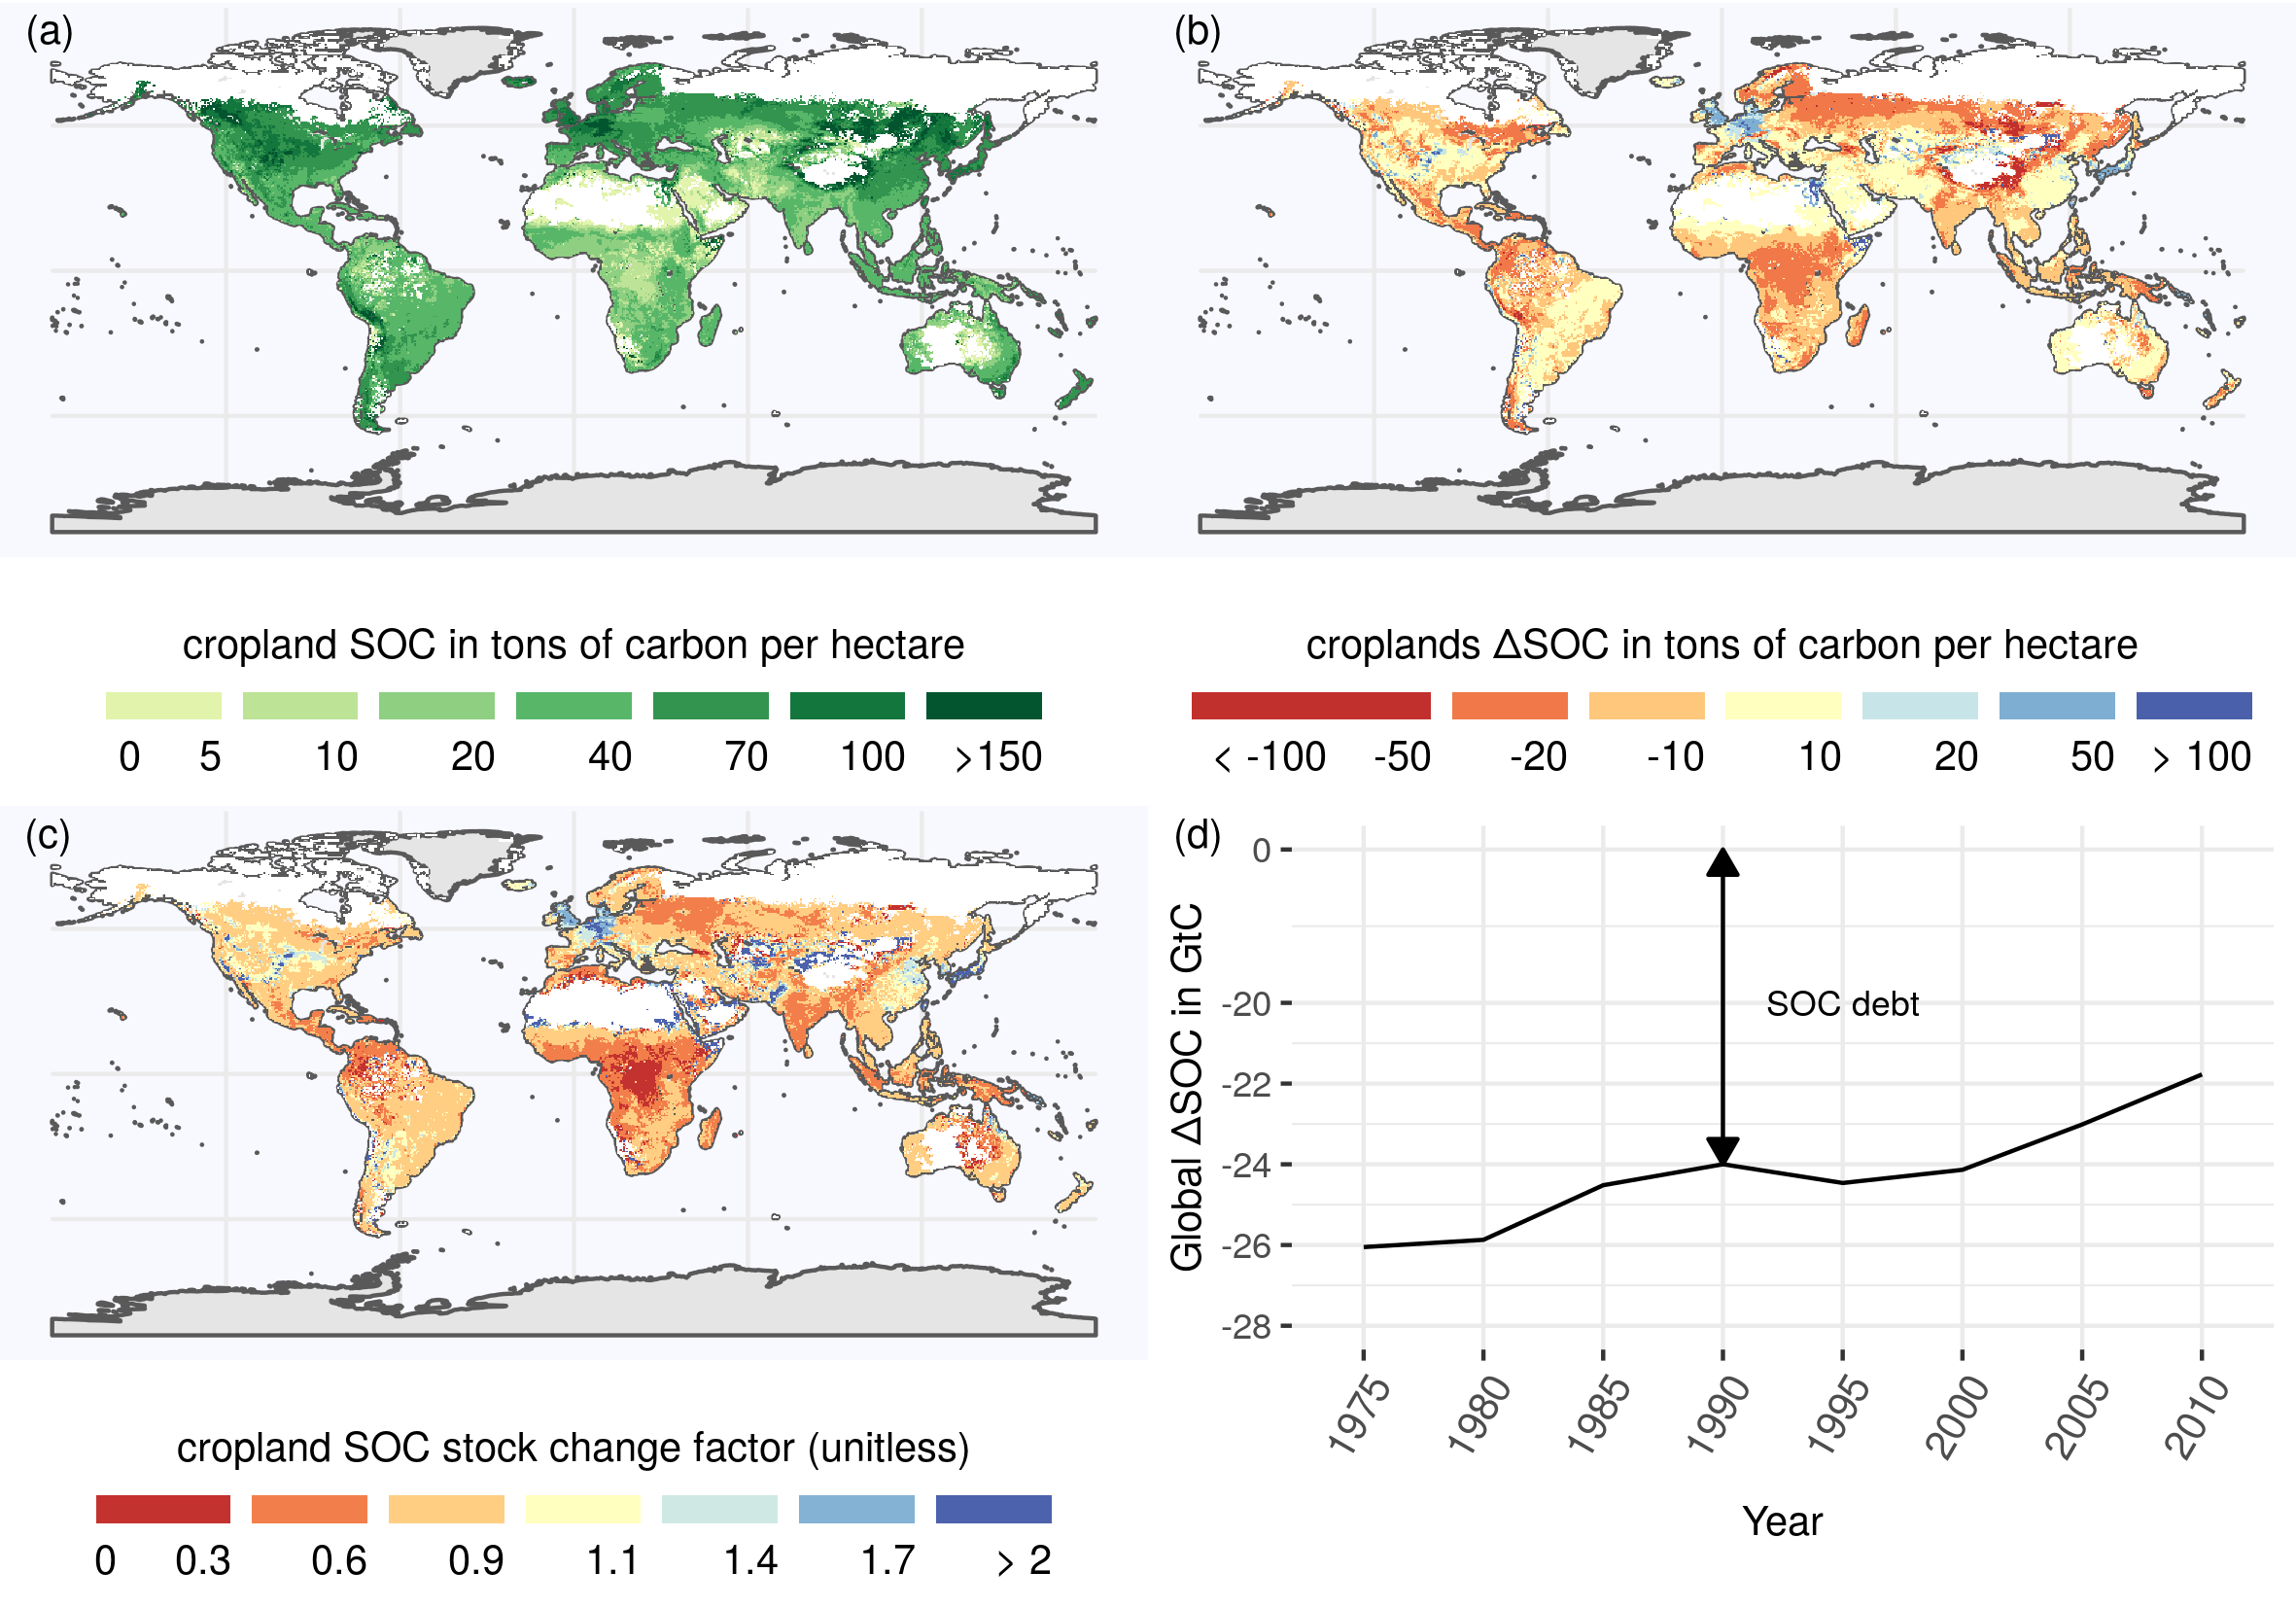
\includegraphics[width=18cm]{../ResultNotebooks/Output/Images/4panelfigure} \caption{(a) ... , (b) ... , (c) ... , (d) ... .}\label{fig:SOCmaps}
\end{figure}

\newpage

\hypertarget{comparison-of-stock-changes-factors}{%
\subsection{comparison of stock changes factors}\label{comparison-of-stock-changes-factors}}

\begin{table}

\caption{\label{tab:table}SCF compared to potential natural state}
\centering
\begin{tabular}[t]{l|r|r|r|r}
\hline
  & tropical\_moist & tropical\_dry & temperate\_dry & temperate\_moist\\
\hline
1965 & 0.25 & 0.33 & 0.55 & 0.48\\
\hline
1970 & 0.29 & 0.36 & 0.56 & 0.50\\
\hline
1975 & 0.32 & 0.38 & 0.57 & 0.51\\
\hline
1980 & 0.34 & 0.38 & 0.56 & 0.53\\
\hline
1985 & 0.36 & 0.40 & 0.60 & 0.56\\
\hline
1990 & 0.38 & 0.42 & 0.63 & 0.58\\
\hline
1995 & 0.40 & 0.45 & 0.63 & 0.59\\
\hline
2000 & 0.42 & 0.47 & 0.64 & 0.60\\
\hline
2005 & 0.45 & 0.54 & 0.69 & 0.65\\
\hline
2010 & 0.50 & 0.58 & 0.73 & 0.67\\
\hline
\end{tabular}
\end{table}

\begin{table}

\caption{\label{tab:table2}SCF compared to IPCC Tier 1}
\centering
\begin{tabular}[t]{l|l|l|l|l}
\hline
Data1 & tropical\_moist & tropical\_dry & temperate\_dry & temperate\_moist\\
\hline
IPCC2006 & 0.48 & 0.58-0.64 & 0.80 & 0.69\\
\hline
IPCC2019 & 0.83 & 0.92 & 0.76-0.77 & 0.69-0.70\\
\hline
model & 0.5 & 0.58 & 0.73 & 0.67\\
\hline
\end{tabular}
\end{table}

\newpage

\hypertarget{global-agricultrual-carbon-flows-and-stocks}{%
\subsection{global agricultrual carbon flows and stocks}\label{global-agricultrual-carbon-flows-and-stocks}}

\newpage

\hypertarget{discussion}{%
\section{Discussion}\label{discussion}}

Big points:

\begin{itemize}
\item
  SOC initialization is bad (Task: find a better representation)
\item
  natural land representation is lacking proper parametrization of natural input (n, lg content of litterfall) (--\textgreater{} ask Christop again)
\item
  boreal zone and dry regions are not well represented (maybe because of the bad parameterization of the soil model for natural soils)
\item
  As pointed out by Keel (2017), Smith (2019) the results might be highly sensitive to carbon input calculations more precisly to below and above ground residue carbon estimates derived from harvested quantities. It has been questioned, that below ground residues might increase with a fixed root:shot ratio (maybe specifically in high end farming systems (?)). Following this argumentation SOC results shown in this study might especially in high-yielding farming system (europe etc.) overestimate actual SOC stocks.
\item
  fertilizer interaction (--\textgreater{} ask LPJmLer again)
\item
  ``The Tier 2 method does not simulate C change but simply calculates an annual C stock change from the
  current C stock to the future steady-state soil C stock calculated based on current conditions.'' Leading to the fact that our total stock results are highly uncertained.
\item
  diaggregation of manure with urban area is leeding to a lot of displaced manure (?) that is cut off
\item
  mismatches between FAO/LUH
\end{itemize}

Shortcommings:

\begin{itemize}
\item
  pasture dynamics are neglected and treated as natveg / Note that manure excreted to pastures is neglected within these analysis, since we focus purely on cropland dynamics.
\item
  no tillage adaptaion is neglected on cropland. Pastures are assumed to be not tilled at all (propably at least heavy managed pastures are tilled with some rotation)
\item
  irrigated areas are no crop specific and growing periods are not considered (since this is very complex to calculate average growing periods). Crop specific growing periods might be possible using LPJmL data.
\item
  Carbon displacement via leaching and erosion is neglected in this study.
\item
  Non-net/Gross land use transitions are not tracked in this study.
\item
  Within cropland we do not track area transitions, but rather look at statistical distributions of the crop functional types. Due to crop rotations and missing data on crop specific distributions, these transitions would be any way rather uncertain.
  \newpage
\end{itemize}

\conclusions

The conclusion goes here.
You can modify the section name with \texttt{\textbackslash{}conclusions{[}modified\ heading\ if\ necessary{]}}.
\newpage




\codedataavailability{use this to add a statement when having data sets and software code available} %% use this section when having data sets and software code available



%%%%%%%%%%%%%%%%%%%%%%%%%%%%%%%%%%%%%%%%%%
%% optional

%%%%%%%%%%%%%%%%%%%%%%%%%%%%%%%%%%%%%%%%%%
\appendix
\section{Figures and tables in appendices}
\subsection{Option 1}

If you sorted all figures and tables into the sections of the text, please also sort the appendix figures and appendix tables into the respective appendix sections.
They will be correctly named automatically.

\subsection{Option 2}

If you put all figures after the reference list, please insert appendix tables and figures after the normal tables and figures.

\texttt{\textbackslash{}appendixfigures} needs to be added in front of appendix figures
\texttt{\textbackslash{}appendixtables} needs to be added in front of appendix tables

Please add \texttt{\textbackslash{}clearpage} between each table and/or figure. Further guidelines on figures and tables can be found below.
Regarding figures and tables in appendices, the following two options are possible depending on your general handling of figures and tables in the manuscript environment:
To rename them correctly to A1, A2, etc., please add the following commands in front of them:
\noappendix

%%%%%%%%%%%%%%%%%%%%%%%%%%%%%%%%%%%%%%%%%%
\authorcontribution{Karstens wrote code and paper build on work of Bodirsky. Bodirsky, and Popp revised paper.} %% optional section

%%%%%%%%%%%%%%%%%%%%%%%%%%%%%%%%%%%%%%%%%%
\competinginterests{The authors declare no competing interests.} %% this section is mandatory even if you declare that no competing interests are present

%%%%%%%%%%%%%%%%%%%%%%%%%%%%%%%%%%%%%%%%%%
\disclaimer{We like Copernicus.} %% optional section

%%%%%%%%%%%%%%%%%%%%%%%%%%%%%%%%%%%%%%%%%%
\begin{acknowledgements}
Thanks to the rticles contributors!
\end{acknowledgements}

%% REFERENCES
%% DN: pre-configured to BibTeX for rticles

%% The reference list is compiled as follows:
%%
%% \begin{thebibliography}{}
%%
%% \bibitem[AUTHOR(YEAR)]{LABEL1}
%% REFERENCE 1
%%
%% \bibitem[AUTHOR(YEAR)]{LABEL2}
%% REFERENCE 2
%%
%% \end{thebibliography}

%% Since the Copernicus LaTeX package includes the BibTeX style file copernicus.bst,
%% authors experienced with BibTeX only have to include the following two lines:
%%
\bibliographystyle{copernicus}
\bibliography{SOCbudget.bib}
%%
%% URLs and DOIs can be entered in your BibTeX file as:
%%
%% URL = {http://www.xyz.org/~jones/idx_g.htm}
%% DOI = {10.5194/xyz}


%% LITERATURE CITATIONS
%%
%% command                        & example result
%% \citet{jones90}|               & Jones et al. (1990)
%% \citep{jones90}|               & (Jones et al., 1990)
%% \citep{jones90,jones93}|       & (Jones et al., 1990, 1993)
%% \citep[p.~32]{jones90}|        & (Jones et al., 1990, p.~32)
%% \citep[e.g.,][]{jones90}|      & (e.g., Jones et al., 1990)
%% \citep[e.g.,][p.~32]{jones90}| & (e.g., Jones et al., 1990, p.~32)
%% \citeauthor{jones90}|          & Jones et al.
%% \citeyear{jones90}|            & 1990

\end{document}
